\documentclass{article}

% if you need to pass options to natbib, use, e.g.:
% \PassOptionsToPackage{numbers, compress}{natbib}
% before loading nips_2018

% ready for submission
%\usepackage{nips_2018}

% to compile a preprint version, e.g., for submission to arXiv, add
% add the [preprint] option:
\usepackage[preprint]{nips_2018}

% to compile a camera-ready version, add the [final] option, e.g.:
% \usepackage[final]{nips_2018}

% to avoid loading the natbib package, add option nonatbib:
%\usepackage[nonatbib]{nips_2018}

\usepackage[utf8]{inputenc} % allow utf-8 input
\usepackage[T1]{fontenc}    % use 8-bit T1 fonts
\usepackage{hyperref}       % hyperlinks
\usepackage{url}            % simple URL typesetting
\usepackage{booktabs}       % professional-quality tables
\usepackage{amsfonts}       % blackboard math symbols
\usepackage{nicefrac}       % compact symbols for 1/2, etc.
\usepackage{microtype}      % microtypography
\usepackage[english,ruled,lined]{algorithm2e}
\usepackage{amsmath}
\usepackage{graphicx}
\usepackage{caption}
\usepackage{subcaption}
\hypersetup{
    colorlinks=true,
    linkcolor=blue,
    filecolor=magenta,      
    urlcolor=cyan,
}
\bibliographystyle{unsrtnat}


\title{Outcome Prediction for Stock Data}

% The \author macro works with any number of authors. There are two
% commands used to separate the names and addresses of multiple
% authors: \And and \AND.
%
% Using \And between authors leaves it to LaTeX to determine where to
% break the lines. Using \AND forces a line break at that point. So,
% if LaTeX puts 3 of 4 authors names on the first line, and the last
% on the second line, try using \AND instead of \And before the third
% author name.

\author{
  Abel Sapirstein\thanks{Use footnote for providing further
    information about author (webpage, alternative
    address)---\emph{not} for acknowledging funding agencies.} \\
  Department of Computer Science\\
  Harvey Mudd College\\
  Claremont,CA ,91711 \\
  \texttt{asapirstein@hmc.edu} 
}

\begin{document}
% \nipsfinalcopy is no longer used

\maketitle

\begin{abstract}
This work seeks to explore how different cluster algorithms on stock data to automate prediction. K Means and Expectation Maximization are explored and rejected as potential choices. We postulate a hybrid supervised/unsupervised learning schema with a more complex clustering approach that depends on function distance rather than Euclidean distance and instance instance specific clusters.  
\end{abstract}

\section{Introduction}

Outcome prediction and optimization  of partially complete data is a holy grail of sorts. The premise is a simple one, that future behavior of an objective  can be predicted by observing past behavior and current situations. Mathematicians have proposed several solutions to this problem and there currently exist many tools that predict specific types of outcomes quite well. Such tools have broad reaching implications ranging from improving intensive care outcomes(\cite{meiring}) to making lucrative financial choices (\cite{gerlein}). 

Machine Learning is divided into supervised, where labels are supplied, and unsupervised, where labels are not (\cite{murphy}).This paper will focus on using clustering algorithms to automatically label data, which, having been labeled and approved, can then be passed to supervised learning algorithms, such as neural networks. The effectiveness of such clustering schema was assessed on their ability to accurately predict significant behavior in their constituents.Other mechanism are needed to accurately predict behavior when this approach fails.

Stock data provides an easily accessible numeric data with a clear application . Predicting future behavior of stocks has long been the aim of traders, but only recently have accurate algorithmic tools emerged. There are several issues with stock data that can prevent classical regression tools from generating accurate prediction of behaviors. However, a clustering approach that automates labelling is appealing because it would allow for use of more advanced and accurate models of supervised learning. 

There is ample past and current literature on both clustering approaches and advanced supervised learning approaches. We chose to implement a hybrid approach including K Means clustering (\cite{murphy}) with a non-Euclidean distance metric,dynamic time warping, and a Markov Chain.We hypothesized that the combination of a clustering algorithm to automate trend labeling and a supervised machine learning approach, would be able to predict market behavior at a rate significantly higher than our previous attempts at stock prediction using a cluster approaches with Euclidean distance metric.  


\section{Materials and Methods}
\subsection{Data and Ridge Regression}
\subsubsection{Training Data}
Training data was composed of the components of the Standard and Poor’s 500 index (SP500) and was taken from January 1st , 2015  until the end of 2018. There are 500 large and medium cap components to the SP500 . This particular index is of interest to us because it is a barometer for the general health of the US economy. Each stock was broken into quarterly earnings reports. The rationale for this particular choice was that market behavior for a specific day was subject to momentum from the previous four weeks. Furthermore, markets are often subject to large events that affect all components of the specific sectors of the SP500. 
To minimize both the affect of large market events and still provide an accurate representation of the stocks behavior over the quarter, we fit a tenth-degree polynomial to each quarter’s closing price values. This was done via ridge regression against the normalized initial value—the first day of the quarter always had an initial value of 1.00. Furthermore, to better explain the minutia of stock behavior, we broke down the SP500 into industrial sectors (Appendix A) and ran the following models on each individual sector. We though that large market events, that impacted the cost to a particular industry of doing business would be felt strongly in that sector, but not in other sectors, hence the sector based approach. 
Data was gathered from the Investors Exchange via their API and looked only at the close price for each day. It is worth noting that though the components of the SP500 have changed since 2015.For simplicity's sake, however, the data used queried only current components of the SP500.
\subsubsection{Testing Data}
After models were created, they were validated against a selection of sector stocks that are not included in the  SP500 index. Additionally the model was validated on SP500 data taken over a different window. If a model was trained on a specific industrial sector, we would expect that the accuracy of the model on the testing data, on stocks in the same sector, would be approximately equal to that of the training set. The same method was used to generate data 

\subsection{Algorithms}
\subsubsection{Fréchet Distance}
\begin{equation}
    \label{frechet}
    F(A,B) = \inf \max_{t \in [0,1]}\left[||A(\alpha(t))-B(\beta(t))||^2_2 \right]
\end{equation}
As proposed by Eiter and Mannila (\cite{eiter}), the discrete Fréchet distance is the minimum cord length needed to traverse a pair of curves(\ref{frechet}). Here $\alpha$ and $\beta$ are reparameterization functions that take the timescale of $A$ and $B$ respectively and map it onto the $[0,1]$ interval. The Fréchet distance is a better similarity metric for this application because it will group curves that behave relatively similarly over together and heavily penalize for disjointed regions. we used Charles Jekel's implementation of Eiter and Minnila's discrete Fréchet distance, which runs in $O(NM)$ time, where $N$ is the size of $A$ and $M$ is the size of $B$. 
\subsubsection{K Means}
\begin{equation}
    \label{kmeans:objective}
    RSS_k = \sum_{\vec{x} \in \vec{\omega_k}}|F(x,\mu_k)|^2\text {   with   } \mu_k \text{as closest cluster}
\end{equation}
K means is one of the most widely used clustering algorithms, with applications ranging from cyber-profiling (Riadi et al., 2016)  to epidemiology (Haughen et al. 2019). It works by creating centroids and grouping points to the centroid according to a distance metric. In this study we elected to use the Fréchet distance because the Euclidean distance metric did not sufficiently capture the complexities of our data. The objective function for K means (\ref{kmeans:objective} ) seeks to minimize the total residual sum of squared errors. This is done iteratively via the approach outlined in Algorithm 1. Once the objective function cannot be minimized any further, the algorithm has converged. This algorithm was implemented in Python (3.7) using the NumPy, SciPy, and similiaritymeasures  packages. Run time is suboptimal because the Fréchet distance metric requires significant computational time.  
\begin{center}
\begin{algorithm}
 \textit{initialize} $\mu_k$ \;
 \Repeat{\textit{converged} or $(\mu_k)_n = (\mu_k)_{n+1}$}
   {Group each point to nearest cluster center: $z_i = \arg \min_k F(x_k,\mu_k)$\;
   Average all points in grouping and update cluster: $\mu_k = \frac{1}{N_k}\sum_{i:z_i = k} X_i$}
  
  \caption{K Means or Hard EM, from Murphy}
\end{algorithm}
\end{center}
One of the major advantages to using this approach was that we were able to analyze the patterns that were unique to each sector. As demonstrated below, this allows us to better express the minuta of market forces in a particular stock. 
\begin{figure}[ht]
\centering
\begin{subfigure}{.45\textwidth}
  \centering
  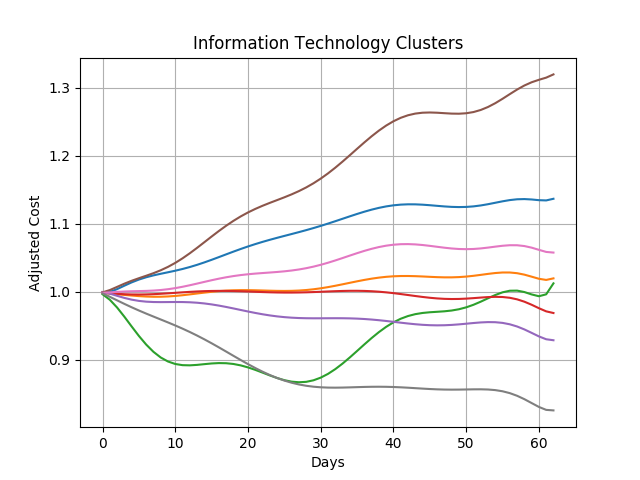
\includegraphics[width=\linewidth]{informationtechnology.png}
  \caption{}
  \label{kmeans:a}
\end{subfigure}%
\begin{subfigure}{.45\textwidth}
  \centering
  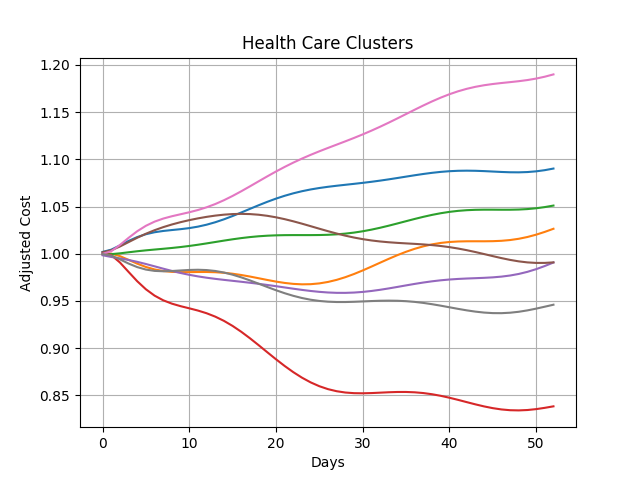
\includegraphics[width=\linewidth]{healthcare.png}
  \caption{}
  \label{kmeans:b}
\end{subfigure}
\caption{Generated K-means centroids for both Health Care and Information Technology Sectors. Note the difference in each sectors cluster}
\label{markov}
\end{figure}
\subsubsection{Dynamic Time Warping}
Fast dynamic time warping (DTW) is a widely used metric for measuring the similarity between two time series by finding an optimal warping path.(\cite{salvador}) This is of interest to us because we assume that certain market stocks are predictors of others, e.g.  an increase in silica costs may lead to increase profits for silica manufactures, while decreasing the value of technology stocks. By comparing two sets polynomial representations of a particular stock—each set contains several polynomial expressions of quarter behavior— we could decide if one time series was an approximately phase shifted version of the other. By calculating dynamic time warping for each stock of interest, we could predict the unique combination of stocks that might have a significant predicting properties for the particular stock of interest. For each stock, the DTW comparison was performed against sector components.  
\subsubsection{Prediction}
Prediction of individual stock behavior (simple prediction) was done via a Markov Chain. The initial states were generated clustering the price and volume data from input data (5 days). Final states were determined by clustering and labeling the previously fit polynomial representation of the continuation of the input data.  The stochastic matrix was generated by observing the frequency with which an initial states led to a final state. Simple prediction simply selected the most likely quarter behavior based on the 5 day behavior using the Markov Chain of events. 
Prediction was done by combining simple prediction and dynamic time warping. DTW prediction consisted of finding ‘predictor stocks’ for our stock of interest and simply prediction those stocks. The DTW prediction weighted each ‘predictor stock’ based on its distance from our stock of interest. Shorter distances were given higher weights. Final prediction was done by combining DTW prediction and the simple prediction, weight was determined by the $\ell_2$ norm of each vector. An example of this combination is shown in figure \ref{3m}.
\begin{figure}
    \centering
    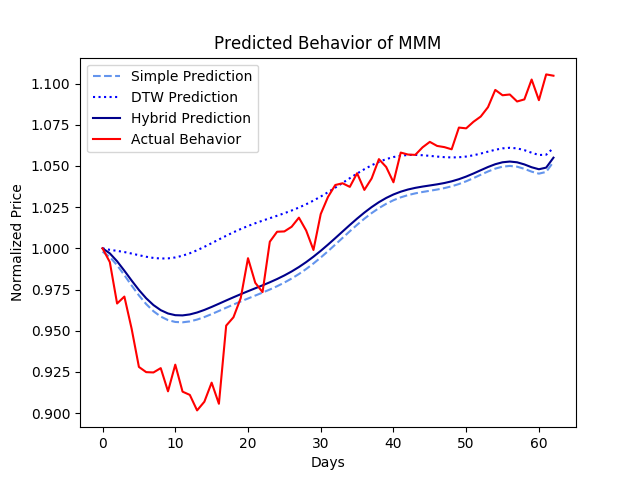
\includegraphics[width = .5\textwidth]{4.png}
    \caption{Simulated Behavior of 3M for the first quarter of 2017}
    \label{3m}
\end{figure}


\subsection{Analytic Tools}
We assessed our model based on how accurately it was able to predict stock behavior at 60 days, given the previous 5 days of data. This was done by predicting each stocks behavior in our training set and testing and subtracting the actual behavior from the predicted behavior. We graphically analyzed the data and calculated critical thresholds for error bounds. 

\section{Results}

K means was run with 8 clusters for both the day and quarter behavior. This number is relatively small because we did not want to potentially over fit the data and wanted to highlight ubiquitous trends. We observed significant intersectoral behavior, indicating that our approach to using a sector specific metric was valid. We predicted 2667 of our 5000 (53\%) training points   to within 5\% yield correctly. An example of a fairly normal prediction is included in figure \ref{3m}, note that in this example the DTW prediction is positive to the overall outcome. In most cases that were accurate to 5\%, the DTW approach is positive, however in a significant fraction of the cases that improperly predicted the effect of similar latent stocks. About 7\% of the predictions were off by more than 50\%.  The distribution of errors is show in figure \ref{errors}. 
\begin{figure}[ht]
    \centering
    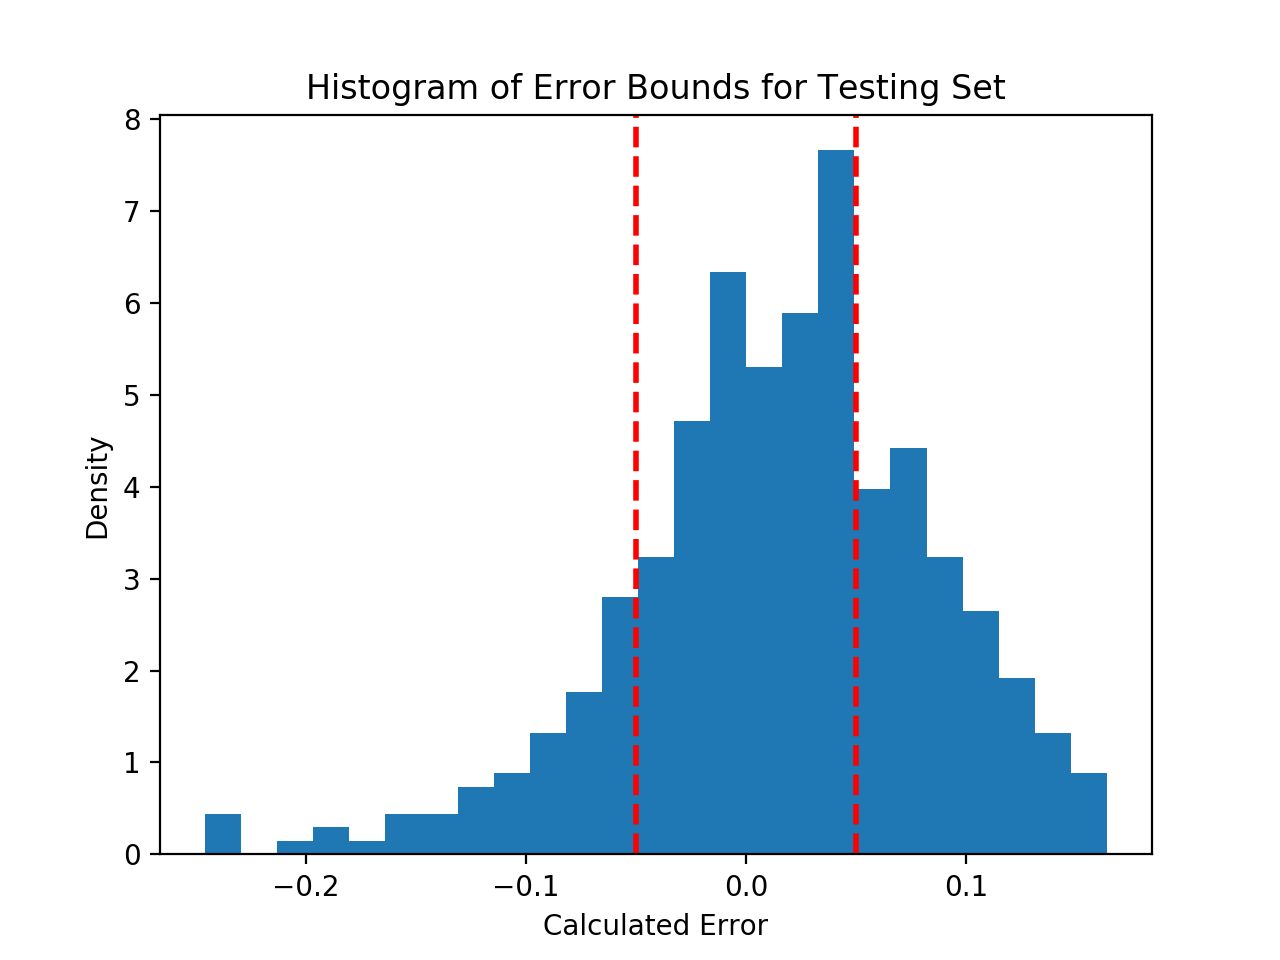
\includegraphics[width = .5\textwidth]{errors.png}
    \caption{Distributions of Errors in Prediction. Red lines represent the 5\% error bound}
    \label{errors}
\end{figure}
\section{Discussion}
	Though this model is not perfect, it represents a significant improvement over our previous attempts at stock prediction. By using the Fréchet distance rather than the $\ell_2$ norm we were able to more accurately predict the behavior at 60 days. This is likely due to a more appropriate metric for assessing similarity. Additionally the inclusion of similar stocks, through dynamic time warping reduced the error associated with prediction by a small but significant amount (1.4\%). Furthermore taking a sector specific approach to this problem allowed us to better train our model to tune into market events that actually impacted that sector. We used very low dimension time series data for this project, following the same method but including other factors that impact the market would be one possible way to improve the predictive accuracy. The most significant sources of error in this iteration of the project was the polynomial regression and the poor predictive power of a simplistic Markov Chain. 
\subsection{Markov Errors}
Interestingly, we observed similar error patterns across the sectors that hinged upon the sparsity of the transition matrix that frequency analysis generated. Because we used very little data, about 8.5\%, of our final desired data, the stochastic matrix was not sparse. In the Markov Chain below, this manifests itself as having many final states connected to an initial state, each with a relatively low probability. This presents a problem because we are seeking to maximize the likelihood that a particular initial state will lead to its predicted final state. Having a low probability of reaching many states, without a particularly strong prediction for any one final state, dramatically harms the predicting power of such an approach.
\begin{figure}[ht]
\centering
\begin{subfigure}{.5\textwidth}
  \centering
  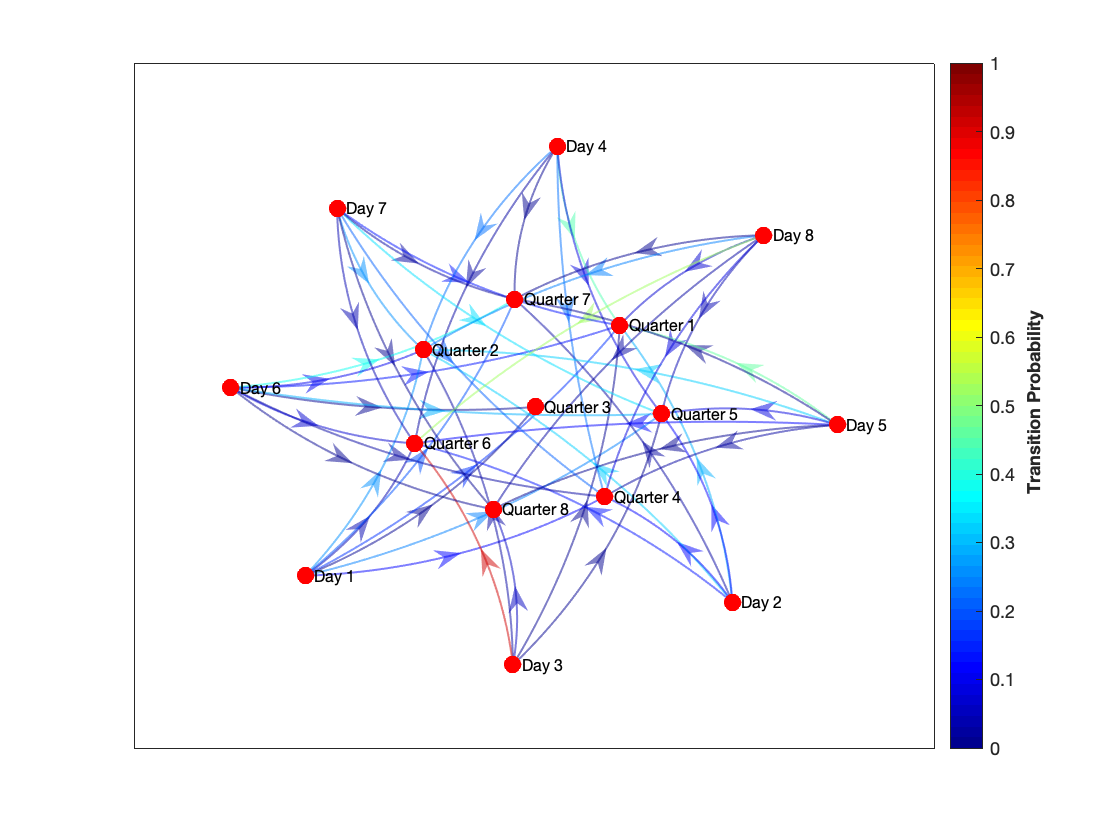
\includegraphics[width=\linewidth]{markov_model.png}
  \caption{Generated Markov Chain}
  \label{markov:a}
\end{subfigure}%
\begin{subfigure}{.5\textwidth}
  \centering
  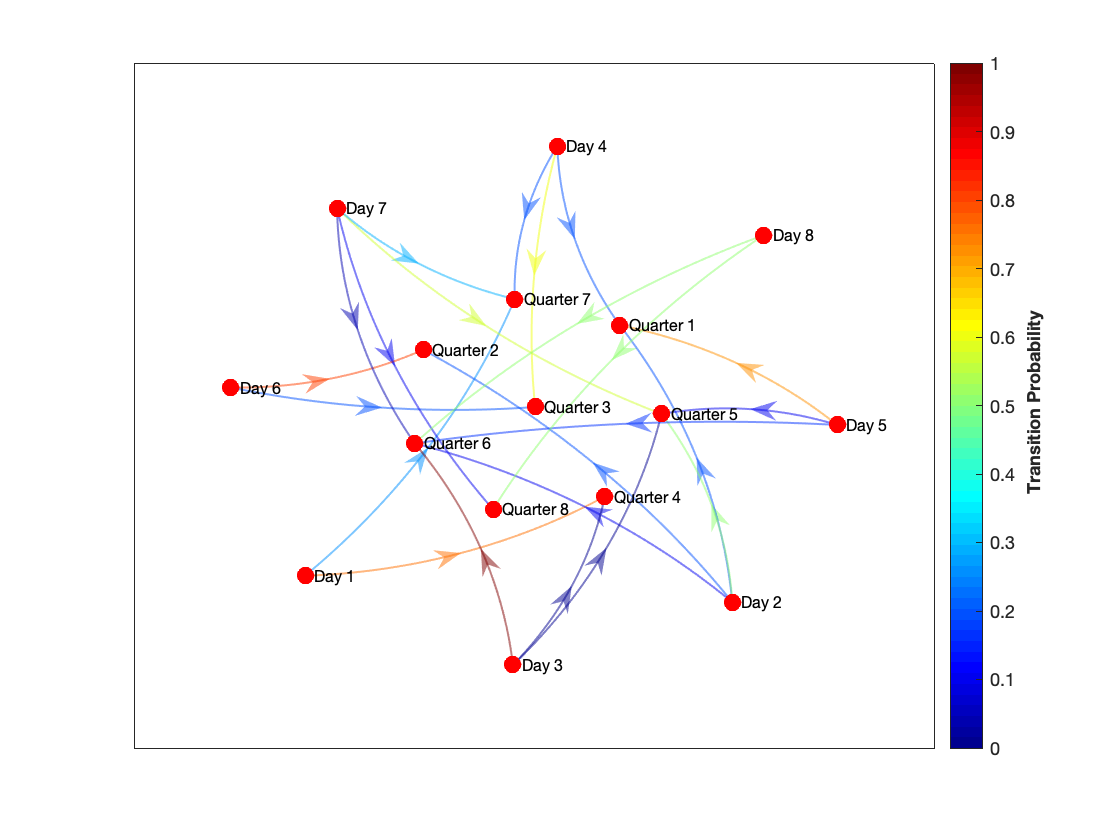
\includegraphics[width=\linewidth]{ideal.png}
  \caption{Ideal Markov Chain, Sparser than \ref{markov:a}}
  \label{markov:b}
\end{subfigure}
\caption{Generated and Ideal Markov Chains;low probability events are indicated in blue, are high-probability is yellow/red. Note that the generated model does not have very many high probabiltiy events, and as such has minimal predicting power}
\label{markov}
\end{figure}
\subsection{Runtime Issues}
Runtime proved to be a significant downsides, our clustering approach relied on a distance metric that required $O(n^3)$ steps and the dynamic time warping also required $O(n^3)$ steps. We had originally hoped to optimize the number of each clusters, experimenting with the appropriate values for each of the two versions, in hopes of getting a sparser stochastic matrix, as outlined in the above paragraph. However because training a single model took upwards on 4 days on the hardware available to us, we were unable to do so. There are ample opportunities for improving the training runtime of the algorithm, but we wished to refrain from devoting a significant portion of our thought to the task until the algorithm was further validated. The actual prediction step of the algorithm does not have the same run-time limits as the training phase.

\subsection{Planned Next Steps}
We had originally planned to test what fraction of the data was needed to generate a more sparse matrix. For example if we include 10 days of data rather than 5, how does the model respond. However, as mentioned above, we were unable to vary these parameters to the degree that we would have liked. 
\section{Conclusions}
This model does, for certain patterns, perform quite well. However these patterns are yet unbeknownst to us. If we can ascertain when the model performs well than we could develop an investment strategy that hinged upon the behavior that the model works well for. Furthermore there is a clear pattern in the stocks that are predicted with large error bounds. When a stocks behavior deviates considerably— greater than 25\% —from others within its sector our model amplifies this deviation improperly and predicts the movement of the stock to be opposite to the true movement of the stock. 

There are many approaches to predicting time-series data, including stocks. After this foray into predicting SP500, it seems a pattern driven approach might be the most suitable. This model can predict certain patterns with remarkable precision, given only a small amount of data. Another set of models— that do not hinge on the same set of assumptions—is needed to fill in the gaps of this model. 

\bibliography{midterm}
\section*{Appendix A}
\begin{center}
    \begin{table}[ht]
\begin{tabular}{ll}
\textbf{Sector}        & \textbf{Number of Components} \\
Consumer Discretionary & 64                            \\
Consumer Staples       & 33                            \\
Energy                 & 29                            \\
Financials             & 67                            \\
Health Care            & 62                            \\
Industrials            & 70                            \\
Information Technology & 68                            \\
Materials              & 26                            \\
Real Estate            & 32                            \\
Utilities              & 28                           
\end{tabular}
\end{table}
\end{center}
\section{Data and Code}
All of the data and code used for this project are available on GitHub. 

\newpage
\end{document}
